\svnkwsave{$RepoFile: siminos/spatiotemp/chapter/reportMNG.tex $}
\svnidlong {$HeadURL: svn://zero.physics.gatech.edu/siminos/spatiotemp/chapter/reportMNG.tex $}
{$LastChangedDate: 2019-10-18 20:49:56 -0400 (Fri, 18 Oct 2019) $}
{$LastChangedRevision: 6846 $} {$LastChangedBy: mgudorf3 $}
\svnid{$Id: reportMNG.tex 6846 2019-04-24 15:30:37Z mgudorf3 $}

\chapter{Space-time investigation of \KS\ system}
\label{chap:reportMNG}
% Predrag                                           26 May 2016

\bigskip

\hfill {\large Matthew N. Gudorf <matthew.gudorf@gatech.edu>}


\section{Turbulence? An overview}
\label{sect:MNGintro}

Fluid flows are well described by the Navier-Stokes equation. Instead of
beginning research with a partial differential equation with three
spatial dimensions, it is wiser to begin with simpler partial
differential equation, e.g. ``Navier-Stokes'' in one spatial dimension,
in order to gain some intuition about the larger picture.

\subsection{\KS\ system}
\label{sect:KSsyss}

One of the simplest partial differential equations that exhibits
spatiotemporal chaotic behavior is the \KS\ [henceforth KS]
system\rf{KurTsu76,siv}, which is used to model a number of different
phenomena, such as unstable flame fronts. The equation for the velocity
of such a flame front
$u(\conf, \zeit)$ on a periodic domain, $u(\conf, \zeit)= u(\conf + L,
\zeit)$.
\beq
    u_\zeit + \frac{1}{2}(u^2)_\conf + u_{\conf \conf} + \nu u_{\conf \conf \conf \conf} = 0 \, \quad x \in [0, L]
\eeq
The terms each contribute differently to the dynamics: $u_{\conf \conf}$
contributes to instability, $u_{\conf \conf \conf \conf}$ provides
damping, and $u^2_{\conf}$ transfers energy between large and small
scales (e.g. between Fourier modes with small and large wavenumbers).

The equations can be made dimensionless by scaling out the 'viscosity'
$\nu$ with transformations $\conf \rightarrow \conf\nu^{1/2}, \zeit
\rightarrow \zeit\nu , u \rightarrow u\nu^{-1/2}$. Hence the
\KSe\ takes the non-dimensionalized form:
\beq
     u_\zeit + \frac{1}{2}(u^2)_\conf + u_{\conf \conf}
     + u_{\conf \conf \conf \conf} = 0 \, \quad x \in [0, L\nu^{-1/2}]=[0,2\pi\tildeL]
\ee{ks}
In these dimensionless units, periods of periodic solutions are also
rescaled following the relation: $T_p = \frac{T^{*}_p}{\nu}$.

Possible avenues of study of the equation and its behavior include
varying $L$ while keeping $\nu = 1$, or varying $\nu$ while keeping $L =
1$ or $2\pi$.

The \KS\ equation have a number of different symmetries, namely: spatial
translational invariance, temporal translation invariance, reflection
invariance, and Galilean invariance. In order to exploit the periodicity
of the equations, we recast the field in its Fourier representation
\beq
u(\conf, \zeit) =
\sum_{k = -\infty}^{\infty} \Fu_k e^{iq_kx} \quad \mbox{where } \, q_k = \frac{2\pi}{L}
\,.
\eeq
The \KSe's representation in terms of spatial Fourier modes is then:
\beq
\dot{\tilde{u}}_k = (q_k^2-q_k^4)\Fu_k-i\frac{q_k}{2}\sum_{m=-\infty}^{\infty}\Fu_m\Fu_{k-m}
\,.
\eeq
The hyper-viscosity term $-q^{4}_k$ term, damps the higher modes such
that a truncation of Fourier modes still yields accurate results, however
different numbers of modes can inherently change the nature of the
solution in the asymptotic limit.

One can also look at the antisymmetric subspace of the full \statesp\
defined by $u(\conf,\zeit)=-u(-\conf,\zeit) \in \bbU^+$. The subspace
$\bbU^+$ can be described with the case of purely imaginary Fourier
coefficients $\Fu_k \rightarrow i\Fu_k$, such that the evolution equation
becomes:
\beq
\dot{\tilde{u}}_k
= (q_k^2-q_k^4)\Fu_k-\frac{q_k}{2}\sum_{m=-\infty}^{\infty}\Fu_m\Fu_{k-m}
\,.
\eeq
By doing so, one eliminates the continuous translational symmetry that is
present in the full \statesp\ formulation.

\subsection{Visualizations}
\label{sect:MNGvisual}


There are plenty of ways to visualize the evolution of solutions to the
\KSe, however not all visualizations are equal in terms of insight or
usefulness. In our applications, pretty plots of the spatiotemporal
dynamics of $u(\conf, \zeit)$ are usually not the most useful for further
analysis; projections of trajectories in $\infty$\dmn\ \statesp s are often
more useful.
Furthermore, Poincar\'e return maps often offer more information than the
full \statesp\ pictures, specifically about the fractal structure of
strange attractors.

\subsection{\Eqva}
\label{sect:MNGeqva}

By setting $u_t = 0$ and integrating over \refeq{ks} once, one arrives at
\beq
\frac{1}{2}u^2 + u_\conf + u_{\conf \conf \conf} = c
\,,
\eeq
which we can write as $3$ ODEs in $\conf$,
\beq
u_\conf = v ,\quad v_\conf = w , \quad w_\conf = u^2 - v -c
\,.
\eeq
This equation exhibits a reversal symmetry, $\conf \rightarrow
-\conf , u \rightarrow -u , v \rightarrow v , w \rightarrow -w$.
The third equation can be rewritten as
\beq
(u+w)_x = u^2 - c
\,.
\eeq
For us the interesting dynamics occurs for $c>0$. The sets of bounded
solutions are complex and fractal in nature. The equilibria in this
regime are given by $c_+ = (\sqrt{c},0,0)$ and $c_- = (-\sqrt{c},0,0)$.
One can acquire the Floquet multipliers by linearizing the flow around
one of the equilibria; the opposite equilibria will exhibit a reversed
stability profile due to the 'time' reversal symmetry previously
mentioned.

For fixed system size $L$, the only surviving equilibria have periodicity
equal to $L$. The corresponding equilibrium condition is then:
\beq
q^2_k (1-q^2_k)\Fu_k + i\frac{q_k}{2}\sum_{m=-\infty}^{\infty}\Fu_m \Fu_{k-m} = 0
\,.
\eeq
On a finite periodic domain, the spatially periodic equilibria have periods which
are multiples of $L$. There is a bifurcation every time $\tildeL$
crosses and integer value, i.e. when $\tildeL = n$, $n$-cell states are
generated through pitchfork bifurcations.
    %\PC{2016-08-15}{\tildeL\ has not been defined anywhere}

In the full \statesp\ they form an invariant circle due to translational
invariance.

In the antisymmetric subspace $\bbU^+$ the aforementioned equilibria
correspond to two points, which are half-period translations of each
other:
            %\PC{2016-08-08}{you have not yet defined `the antisymmetric
            %subspace', this remark cannot be understood here..}
\beq
\nonumber
u(\conf, \zeit) = -2\sum_k \Fu_{kn}\sin{(kn\conf)} \quad \mbox{where,} \quad \Fu_{kn} \in \mathbb{R}
\eeq
The spatially periodic solutions is finite, due to the finite allowance
of zeros of analytic functions on a finite-dimensional compact manifold.

\subsection{Time-stability analysis: why flame fronts flutter?}
\label{sect:MNGtimeStab}


The time-evolution stability matrix evaluated at an \eqv\ $\ssp_q$ is
constant, therefore the Jacobian follows by exponentiation:
\beq
\nonumber
\J^{t}\,(\ssp_q) = e^{At} \quad \mbox{where,} \quad A = A(\ssp_q)
\,.
\eeq
For small $\tildeL<1$, $u(\conf, \zeit) = 0$ is a globally attractive
stable equilibrium. As $\tildeL$ increases, there is a sequence of
bifurcations that affects the dynamics in an unstable and `turbulent'
manner.

Long wavelength perturbations are linearly unstable, while short
wavelength perturbations are strongly contractive. For example, an
equilibrium solution can be very unstable in 5 eigen-directions, but with
strong contraction in higher, stable eigen-directions. In particular, the
equilibrium $u(\conf,\zeit)=0$ has Fourier modes as linear stability
eigenvectors. The Fourier modes who satisfy $|k|<\tildeL$ are unstable.
The most unstable mode has $k$ closest to $\frac{\tildeL}{\sqrt{2}}$.

Truncation of higher Fourier modes can by justified through the following
analysis: If the initial $\Fu_k$ are small then the bilinear term $\Fu_m
\Fu_{k-m}$ can be neglected. Then the equations become decoupled linear
equations whose solutions are exponentials. There are then a finite
number of modes growing with time. These unstable modes excite the higher
modes through the bilinear term. However, higher modes are highly damped.
Therefore the intermediate wavelengths play an important role in
maintaining a dynamic, on-average equilibrium, but truncation can be
employed so long as all important modes are kept. A consequence of this
is that an infinite-dimensional problem has become finite dimensional.

There is no chance of reversing the evolution because of the high (in
principle infinite) number of highly-contracting modes. The time reversal
turns these into highly unstable modes.

\Eqva\ are important because they play two different roles:
\begin{itemize}
\item More unstable directions implies less time spent by an orbit in its neighborhood.
\item Orbits spend large fractions of time in neighborhoods of equilibria with only a few unstable directions.
\end{itemize}

\subsubsection{Intrinsic parameterization}
\label{sect:MNGintrPar}


The best coordinate system to use are generated by the stable/unstable manifolds. It would be best to find a coordinate transformation to new, curvilinear coordinates where the dynamics take place but it's not known if this can be done, let alone if it can be done globally.

\subsection{Energy budget}
\label{sect:MNGenBudg}


The space average of a function $a(\conf, \zeit)$ periodic on the interval $L$ is given by
\beq
\left<a\right> = \left<a\right>(\zeit) = \frac{1}{L}\oint a(\conf,\zeit)\,dx
\eeq
Total derivatives vanish via spatial periodicity, and integration by parts yields
\beq \nonumber
\left<f_x\right> = 0, \quad \left<f_xg\right> = -\left<fg_x\right>
\eeq
The mean value of time dependent $\left<a\right>(\zeit)$ is given by
\beq
\bar{a} = \lim_{t\to\infty}\frac{1}{t}\int_{0}^{t}\,d\tau \,\left<a\right>
\eeq
The average value of a function on a periodic orbit only requires the
integration over one period. For an equilibrium the time
average is equal to the space average, which is in turn equal to the
value of the function evaluated at the equilibrium.

For the \KSe\ the local velocity square, ${u^2}/{2}$, can be interpreted
as the kinetic energy density when used in the spatial average equation.

Because the Fourier modes are eigenvectors of the translation operator,
the energy is a diagonalized quadratic norm in Fourier space.
\beq
E = \sum_{k=1}^{\infty} E_k , \quad E_k = \frac{1}{2}|a_k|^2
\eeq
By applying a time derivative, a substitution of variables and
integration by parts, one arrives at
\beq
\dot{E} = P - D , \quad P = \left<u^2_x\right>, \quad D = \left<u^2_{xx}\right>
\eeq
As the time averaged energy density on a generic orbit is expected to go
to a constant, on average the power-in $P$ and the dissipation rate$D$
balance each other.

In the Fourier basis the conservation of energy can be written
\beq
\sum_{k=-\infty}^{\infty}\,(q^2_k-q^4_k)\overline{E}_k
\eeq
Therefore $\overline{E}_k$ have to decrease faster than $q^{-4}_k$.
            \PC{2016-08-15}{I disagree (asymptotic bound says nothing
            about small $k$), so I have removed this: ``The active
            Fourier modes can be determined by whether they deviate from
            this bound.''}

\subsection{Numerical methods}
\label{sect:MNGnumMeth}


There are three main methods by which one can attempt to integrate a PDE:
\begin{itemize}
\item Discretize the configuration space by means of a grid of $N$ points
    and approximate the derivatives $u_\conf$, $u_{\conf \conf}$, and
    $u_{\conf \conf \conf \conf}$ with a finite difference scheme of
    appropriate order.
\item Integrate the equations for a finite number of (truncated) Fourier
    modes, paying attention to the stability of the integrator and
    stiffness of the equations.
\item Pseudo-spectral integration of the equations: at each step calculate
    the nonlinear term in configuration space and then bring
    the result back to Fourier space.
            %\PC{2016-08-08}{I thought you compute the nonlinear term in the
            %configuration space, then Fourier transform it?}

\end{itemize}


\section{Summer 2016 Report}
\label{sect:MNGsumm16}

In this report I will describe my efforts towards implementing MATLAB
code that allows for spatial integration of the \KSe. The big caveat is
that I have still not been able to accomplish this, at least as of the
time of the current version of this report.

\subsubsection{\KSe}
\label{sect:MNGkse}


The one spatial dimension \KSe\ is given by
\beq
    u_\zeit + u u_\conf
    + u_{\conf \conf}+\nu u_{\conf \conf \conf \conf} = 0 \,,
    \label{e-MNGre1}
\eeq
The terms of this equation all play different roles: $u_{\conf \conf}$
is an ``anti-diffusion'' term, that pumps energy into the system and
feeds instabilities on large length scales,
$u_{\conf \conf \conf \conf}$ which provides damping on small  length scales, and
the nonlinear, inertial term $u u_\conf$ which transfers energy between
large and small scales. The ``hyper-viscosity" $\nu$ plays through
the dimensionless parameter $\tildeL = L/(2\pi \sqrt{\nu})$ a role analogous
to the role that the Reynolds number $Re$ plays in the Navier-Stokes equation.

When the \KSe\ is taken with spatially periodic boundary conditions
$u(\conf + L, \zeit) = u(\conf, \zeit)$,  $u(\conf, \zeit)$
can be interpreted as  the vertical velocity
field of a ``ring of fire'', produced by a Bunsen burner, for example. A
number of studies\rf{kstroy89,kstroy92,ksgreene88,Mks86,DoLa14}
explore the steady solutions of this system, i.e., where $u_t = 0$.
These solutions are important when viewed from a topological perspective,
as the equilibria play a role in the organization of the \statesp.


\subsection{Time integration}
\label{sect:MNGtimeInt}


In order to get into spatial integration of a time-strip, one must first generate the time strip. Because of the spatial periodicity of $u(\conf, \zeit)$, the time evolution of solutions is best done in Fourier space. The \KSe\ in Fourier space takes the form,

\beq
\dot{\tilde{u}}_k = (q_k^2-q_k^4)\Fu_k-i\frac{q_k}{2}\sum_{m=-\infty}^{\infty}\Fu_m\Fu_{k-m}
\label{e-MNGre2}
\eeq

The term with $-q_k^4$ serves to damp higher Fourier modes, which allows accurate and stable results even when truncating the infinite number of Fourier modes, a notion that makes numerical implementation feasible. Also, because $u(x,t)$ is a physical and hence, a real quantity, there also exists the relation between Fourier coefficients $u_{-k}=u_k^{*}$. Therefore for a truncation that keeps $N$ Fourier modes, we can rewrite the Fourier space equation as,

\beq
\dot{\tilde{u}}_k = (q_k^2-q_k^4)\Fu_k-i\frac{q_k}{2}\sum_{m=0}^{N/2-1}\Fu_m\Fu_{k-m}
\label{e-MNGre3}
\eeq

To integrate this equation numerically, we first start with spatially
discretizing the \KS\ system by Fourier expanding the field
$u(\conf_n,\zeit)= u_n(\zeit)$ over $N$ points of a periodic spatial
lattice $\conf_n = n L/N$,
\bea
  \Fu_k(\zeit) &=& \frac{1}{N} \sum^{N-1}_0 u_n(\zeit) e^{-iq_k\conf_n}
  \,=\, \frac{1}{N} \sum^{N-1}_0 u_n(\zeit) e^{-i 2 \pi k n /N}
  \,,\quad
q_k = \frac{2 \pi k}{L}
\continue
  u_n(\zeit) &=&\sum_{k=-N/2+1}^{N/2}\Fu_k(\zeit) e^{iq_k\conf_n}
    \,=\, \sum_{k=-N/2+1}^{N/2}\Fu_k(\zeit) e^{i 2 \pi k n /N}
\,,
\label{e-MNGre4}
\eea
where $k$ ranges from $-N/2+1$ to $N/2$ due to how MATLAB's Fast Fourier Transform (FFT) handles an even number of configuration space points. In order to have a completely symmetric spectrum, one would need to have an odd number of configuration space points, which depending on the number and size of prime factors, would increase the computation time.

Following in the footsteps of others, MATLAB code \texttt{kursiv.m} originating from Kassam and Trefethen\rf{ks05com}, is adapted in order to provide accurate time-evolution data of $u_n(\zeit)$. The scheme used in this implementation is a combination of two different methods, Exponential Time Differencing (ETD) and Fourth Order Runge-Kutta (RK4) to form a new schema aptly abbreviated ETDRK4. All of this is applied in \texttt{ksint.m} which was written by Xiong and Ruslan. This generates the time evolution data for spatial Fourier modes with $k = \pm 1, \pm 2, \ldots, \pm 15$. The amplitudes for the $k=0$ and $k=-N/2$ ($N$ even), are taken to be zero.

In order to get the correct fields $u$, $u_x$, $u_{xx}$, and $u_{xxx}$,
one must reorder the values produced by \texttt{ksint.m}, this is because
the real and imaginary components of $\Fu_k$ are stored separately in the
array returned by the function. In order to comply with MATLAB's Inverse
Fast Fourier Transform (IFFT), the correct way to order the coefficients,
$\Fu_k$, based on mode number $k$ is,

\begin{tabular}{c||c|c|c|c|c|c|c|c}
\hline
k : & 0 & 1 & ... & N/2 & -N/2+1 & -N/2+2 & ... & -1 \\
\hline
\end{tabular}

The velocity field $u(\conf,\zeit)$ is retrieved via application of
MATLAB's Inverse Fast Fourier Transform (IFFT) on each column of
time-evolution data, which correspond to different times. The first three
spatial derivatives of the velocity field are retrieved through the
spectral method known as spectral differentiation via the equations
     \PC{2016-08-15}{Shouldn't $u_k$ be $\Fu_k$ in \refeq{e-MNGre5}?}
\bea
    u_{\conf}( \conf, \zeit) &=&
                \mathcal{F}^{-1} \left\{i q_k \Fu_k \right\} \,, \quad
    u_{\conf \conf}( \conf, \zeit) =
                \mathcal{F}^{-1} \left\{(i q_k)^2 \Fu_k \right\} \,, \quad \continue
    u_{\conf \conf \conf}( \conf, \zeit) &=&
                 \mathcal{F}^{-1} \left\{(i q_k)^3 \Fu_k \right\} \,, \quad
                 \label{e-MNGre5}
\eea
A  as we shall see in \refsect{sect:MNGspatInt}, the values of the
spatial derivatives on a time strip are required for spatial integration.

The initial conditions for the time evolution of $\PPO{10.2}$ were
provided by Xiong Ding's \texttt{ks22h02t100E.mat}.

\subsection{Spatial integration}
\label{sect:MNGspatInt}

\subsubsection{Fourier expansions}
\label{sect:MNGspatFourier}

In order to begin spatial integration, we will expand the time periodic data generated from time integration into its discretized temporal Fourier modes. First we will start with the expansion of a time periodic function $u(\zeit) = u(\zeit + T)$, in terms of its temporal Fourier modes.

\beq
    u(\zeit) = \sum_{k = -\infty}^{\infty}
    \Fu_k e^{i \omega_k \zeit} \, , \quad \mbox{where }
    \omega_k = 2 \pi k / \period{}
\,.
\label{e-MNGre6}
\eeq

The Fourier coefficients $\Fu_k$ can be retrieved by inverting \refeq{e-MNGre6},
\beq
    \Fu_k = \frac{1}{T} \int_0^{\period{}} d\zeit\ u(\zeit)
            e^{- i \omega_k \zeit}
            \label{e-MNGre7}
\eeq

The discrete version of these relations can be obtained with the approximation $\int_0^T dt \rightarrow \sum_{n=0}^{N-1}\Delta t$, $\Delta t ={T}/{N} $, namely for the discrete Fourier transform,

\bea
    \Fu_k &=& \frac{1}{N} \sum_{n=0}^{N-1} u(t_n) e^{-i \omega_k t_n} \,,
    \mbox{where } t_n = n T / N \continue
          &=& \frac{1}{N} \sum_{n=0}^{N-1} u(t_n) e^{-i 2 \pi n k / N}
          \, , \continue
          &=& \frac{1}{N} \mathcal{F} \{ u (t_n) \} \, ,
\label{e-MNGre8}
\eea
and likewise for the inverse discrete Fourier transform,
\bea
    u(\zeit_n) &=& \sum_{k = - N/2+1}^{N/2} \Fu_k
    e^{i \omega_k \zeit_n} \, \quad \continue
               &=&\, \sum_{k = - N/2+1}^{N/2} \Fu_k e^{i 2 \pi k n / N}
\label{e-MNGre9}
\eea
The next step is to derive the form that \KSe\ takes in terms of spatial Fourier modes. First we define,
\beq
    u^{(0)} \equiv u \, , \quad
    u^{(1)} \equiv u_{\conf} \, , \quad
    u^{(2)} \equiv u_{\conf \conf} \, , \quad
    u^{(3)} \equiv u_{\conf \conf \conf}
\label{e-MNGre10}
\eeq
which allows us to write the \KSe\ as a system of equations,
\bea
    u^{(0)}_{\conf} &=& u^{(1)} \continue
    u^{(1)}_{\conf} &=& u^{(2)} \continue
    u^{(2)}_{\conf} &=& u^{(3)} \label{e-MNGre11} \\
    u^{(3)}_{\conf} &=& - u^{(0)}_{\zeit} - u^{(2)} - u^{(0)} u^{(1)}
                        \nonumber
\,.
\eea
Now we write the equivalent expression in its Fourier representation,
taking into consideration a truncated number of Fourier modes $N$.
\bea
    \frac{\partial}{\partial \conf} \Fu^{(3)}_k &=&
        - i \omega_k \Fu^{(0)}_k
        \, - \Fu^{(2)}_k
        \, - \sum_{m = 0}^{N/2-1} \Fu^{(0)}_{m} \Fu^{(1)}_{k-m}
         \continue
    \frac{\partial}{\partial \conf} \Fu^{(2)}_{k} &=& \Fu^{(3)}_{k} \, , \continue
    \frac{\partial}{\partial \conf} \Fu^{(1)}_{k} &=& \Fu^{(2)}_{k} \, , \label{e-MNGre12} \\
    \frac{\partial}{\partial \conf} \Fu^{(0)}_{k} &=& \Fu^{(1)}_{k} \, , \nonumber
\eea
The rationale behind the truncation in this context is currently not as
solid as opposed to the time-integration of a (spatial Fourier mode
discretization). There is no longer a term in our equations that damps
the higher modes. There isn't any term that provides energy either, but
the damping was a good control of numerical accuracy. Burak has
proposed to introduce an artificial diffusion term of form $\epsilon
u_{tt}^{(3)}$ into the fourth equation in \refeq{e-MNGre11}. In the Fourier
space this would take the form $-e w_k^2 \Fu_k^{(3)}$, where $e$ is known
as an \textit{artificial diffusion constant}. In our numerics, implementing this with
$e=10^{-4}$ produced no significant effect. According to Burak, a value
$e=10^{-4}$ is still a very large value for the artificial diffusion
constant. Therefore, I did not include this term in most of my computations.

\subsubsection{Handling nonlinearity}
\label{sect:MNGnonlin}


The nonlinear term can be handled in a couple of different ways. The first is to directly calculate the convolution sum; this is undesired as it is slow and more importantly does not treat floating-point truncation errors well. The second method is to calculate it via pseudo-spectral method,

\beq
\sum_{m=0}^{N/2-1} \Fu^{(0)}_m \Fu^{(1)}_{k-m} = \frac{1}{N} \mathcal{F} \left\{ u^{(0)} u^{(1)} \right\} .
\label{e-MNGre13}
\eeq

The third option is to calculate it in a fully spectral manner via the circular convolution function included in MATLAB, \texttt{cconv}. It's hard to tell which is the best from looking at the values produced because they are all similar up to numerical accuracy, but I would believe the pseudo-spectral method is the best because of how the circular convolution function works, the lack of speed of the convolution sum.

\subsubsection{Aliasing errors and dealiasing}
\label{sect:MNGalias}

An additional procedure can be applied to the pseudo-spectral method in order to combat what is known as \textit{aliasing}. Aliasing is byproduct of discretization, wherein the amplitude of higher frequency (or similarly high wavenumber) modes can affect the amplitudes of lower modes. The happens when higher modes are misrepresented as lower modes. For $k = -N/2+1, \ldots, N/2$ and  $j \in \mathcal{Z}$,

\bea
e^{\frac{i 2 \pi \left( k+jN \right) }{N}} &=& e^{\frac{i 2\pi k }{N}}*e^{i 2\pi j}\\
 &=& e^{i 2\pi k }. \nonumber
\eea

In order to account for this, one must apply a dealiasing formula to the computation of the pseudo-spectral term. One way of accomplishing this is to zero-pad the corresponding Fourier mode data before computing the IFFT which results in $u^{(0)}$ and $u^{(1)}$. For example, the number of Fourier mode coefficients is increased from $N$ to $2N$ by including $N$ zero-valued coefficients. The IFFT is then applied which produces $u^{(0)}$ and $u^{(1)}$ arrays each of length $2N$. Element wise multiplication is used with these new arrays of length $2N$ to produce an array equal to the product $u^{(0)} u^{(1)}$. The product is then brought back to Fourier space via FFT. The final step is taking the new Fourier mode data, an array of $2N$ Fourier Coefficients, and extracting the coefficients belonging to modes $k = -N/2+1, \ldots, N/2$.

\subsubsection{Numerical integration}
\label{sect:MNGspatInt}

The actual implementation concerning the integration of these equations was to use the MATLAB's stiff-ODE integrator \texttt{ode15s}. This integrator has higher accuracy than some of its counterparts, such as \texttt{ode23s} and \texttt{ode23tb}. The integrator is designed to be used with its own variable step size algorithms in order to deal with the stiffness of equations, however, linearly space steps can be used if so desired. The error tolerances can also be controlled using \texttt{ode15s} while using a variable step size.

so that the relative tolerance is much more useful when dealing with small numbers. If the relative tolerance is set to be too low, accumulated round off errors will dominate the inaccuracy, while if it is set too high the local discretization errors will dominate.

The integrator requires a separate MATLAB file, \texttt{velocityfunction.m} whose input is $\Fu^{(i)}_{k}$, for $i = 0,1,2,3$ according to \refeq{e-MNGre10} and whose output is $\frac{\partial}{\partial \conf}\Fu^{(i)}_{k}$ i.e. it is the implementation of \refeq{e-MNGre12}.

Once the integrator has finished running, my current MATLAB code
\\
\texttt{timeperiodic.m} converts the spatial evolution of the Fourier
coefficients $\Fu_k^{(i)}$ $i = 0,1,2,3$ into the four (discretized)
spatial fields $(u,
u_\conf, u_{\conf \conf}, u_{\conf \conf \conf})$ via the use of
MATLAB's IFFT.

\subsubsection{Spatial integration results}

\begin{figure}[h]
  \begin{minipage}[height=.20\textheight]{.48\textwidth}
    \centering \small{\texttt{(a)}}
    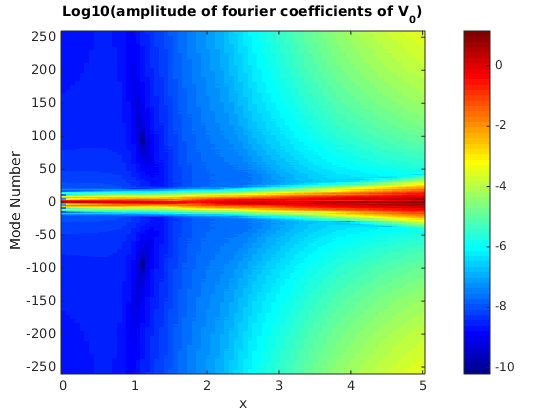
\includegraphics[width=\textwidth,height=.20\textheight]{MNGF0xint5}
  \end{minipage}
  \begin{minipage}[height=.20\textheight]{.48\textwidth}
    \centering \small{\texttt{(b)}}
    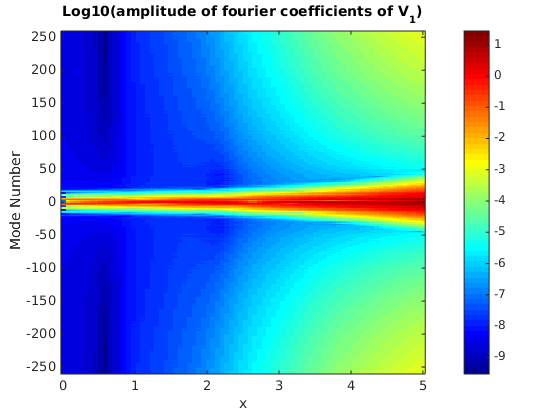
\includegraphics[width=\textwidth,height=.20\textheight]{MNGF1xint5}
  \end{minipage}
  \\
  \begin{minipage}[height=.20\textheight]{.48\textwidth}
    \centering \small{\texttt{(c)}}
    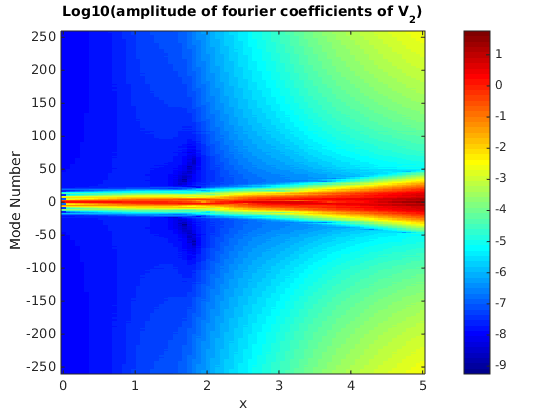
\includegraphics[width=\textwidth,height=.20\textheight]{MNGF2xint5}
  \end{minipage}
  \centering
  \begin{minipage}[height=.20\textheight]{.48\textwidth}
    \centering \small{\texttt{(d)}}
    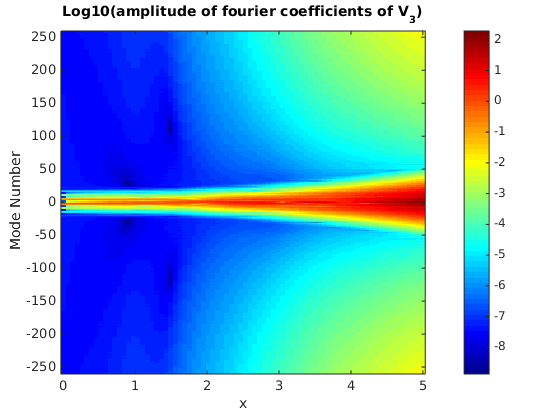
\includegraphics[width=\textwidth,height=.20\textheight]{MNGF3xint5}
  \end{minipage}
   \caption{
   Spatial integration $x=[0,5]$ of temporal Fourier mode amplitudes plotted on a
   $\log_{10}$ scale. (a) $\Fu^{(0)}_{k}$, (b) $\Fu^{(1)}_{k}$,
   (c) $\Fu^{(2)}_{k}$, and (d) $\Fu^{(3)}_{k}$.
            }
  \label{fig:MNGrfig1}
\end{figure}

In its current form, my code is only able to give somewhat sensible
results for short spatial integrations $\conf = [0, L]$, $L = \approx 1$,
where the period of the desired spatially periodic solution is known to
be $L=22$.

This can be seen by looking at the Fourier coefficient amplitudes over
the course of spatial integration, see \reffig{fig:MNGrfig1}. The spectrum
seems to flatten, i.e. the amplitudes of the higher modes grow
dramatically as the spatial extent of the integration is increased.

Considering these limitations I work around the fact that there is a
limited spatial extent on which my integrator seems to work. The way that
I decided to deploy my code was the take increase the number of
configuration space points to 64 in order to increase the resolution and
then integrate the 64 corresponding time-periodic strips over $x = [0,
22/64] = [0, 0.34375]$. I then combine the results such that the
resulting figure attempts to represent spatial integration for $x =
[0,22]$. This technique is not able to exploit the variable step size of
the integrator, as the strips would be of varying sizes and hence the
compilation would not be a very meaningful visualization.

\begin{figure}[h]
  \begin{minipage}[height=.40\textheight]{.35\textwidth}
    \centering \small{\texttt{(a)}}
    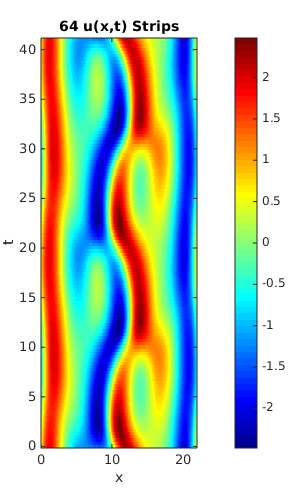
\includegraphics[width=\textwidth,height=.45\textheight]{MNGcompxint22}
  \end{minipage}
  \begin{minipage}[height=.40\textheight]{.35\textwidth}
    \centering \small{\texttt{(b)}}
    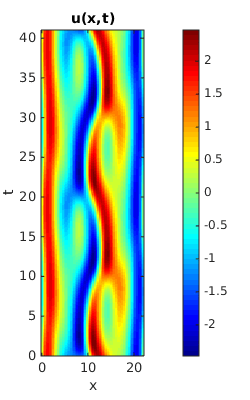
\includegraphics[width=\textwidth,height=.45\textheight]{MNGppo1timeint}
  \end{minipage}
   \caption{Comparison of (a)compilation of 64 spatial integration strips integrated over $x=[0,0.34375]$ and (b) time integration of \PPO{10.2} integrated over time $T = [0,4\,T_{\PPO{10.2}}$, for system size $L=22$}
  \label{fig:MNGrfig2}
\end{figure}

The \reffig{fig:MNGrfig2} is a comparison between the spatial integration
of \refeq{e-MNGre12} using the compilation method I employed in
\texttt{timeperiodic.m} and the time integration of \refeq{e-MNGre3}
using the ETDRK4 numerical scheme implementation of MATLAB file
\texttt{ksint.m}. The behavior of these figures seem to exhibit similar
patterns up to a what appears to be a reflection in the time direction,
implying that there is some unaccounted symmetry. This can be seen by
what I call the ``tails" of the pattern in the middle being pointed in
opposite directions for time and space integration.
        \PC{2016-08-15}{in your {\bf 2016-08-11 Matt} blog entry you seem
        to say that you have now corrected this, and replaced figures by
        the correct ones?}



\subsubsection{Future work and comments}
\label{sect:MNGfuture}

The hope for my code is to be capable of spatial integration of infinite extent. My results are disappointing to me to say the least, having been thrown for loops by what should have been insignificant details, but I hope to use what I've learned in terms of coding in the future.

Some possible means of improving the equations is to look for better ways to dealias the pseudo-spectral term or to use the same method but require it to be more rigorous (e.g. more zero-padding).

Second would be to write an integration scheme that could produce more accurate results. My first thought is to apply the ETDRK4 schema to spatial integration, however, I'm not sure if this would work with a system of equations rather than a single PDE.

Another possible, yet dubious and not warranted, course of action is to find a different way to apply damping in the equations, as the steady growth of the Fourier amplitudes is the main cause of all of my problems.

% Predrag moved this FTnormal.tex to discsymm.tex 2019-03-17
%\section{Appendix : Fourier transforms and normalization factors}
%\label{sect:FTnormal}

\section{Spatiotemporal solutions of \KS}
\label{sect:BeginningsPaper}
To find doubly-periodic spatiotemporal solutions to the \KSe while allowing the domain size,
period, and any extra parameters (e.g. shift due to SO(2) rotations) to change, we use a Fourier-Fourier
basis due to the expected exponential convergence behavior of the (spatiotemporal) Fourier coefficients to zero
if a sufficient number of discretization points is used as the spatiotemporal functions are smooth in space
and time.

\subsection{Kuramoto-Sivashinsky in spacetime}
The Kuramoto-Sivashinsky equation is a dissipative partial differential
equation in one spatial dimension.
In a dimensionless form, it can be written as,
\beq
u_t(\conf,\zeit)
= -u_{\conf \conf \conf \conf,\zeit} - u_{\conf \conf,\zeit} - u u_{\conf,\zeit}
\eeq
The explorations into the geometry of its {\statesp}\rf{SCD07}, the
dimension of a possible inertial manifold\rf{DCTSCD14}, and many other
studies have been done on it as it proves itself an interesting case
study of chaotic dynamical systems in continuous variables. The steady
solutions were studied by Michelson\rf{Mks86} as well as Dong and
Lan\rf{DoLa14} in attempts to categorize the geometry and symbolic
dynamics of solutions on the $T=0$ line. Generally, most studies have
been spatiotemporal, with the time being a continuous parameter that
induces a dissipative semi-flow $t \geq 0$. In this case study, we pose
the problem of finding spatiotemporal invariant solutions by assuming
doubly periodic initial conditions, transforming to a Fourier-Fourier
basis, and then solving the truncated set of nonlinear algebraic
equations

\beq \label{eqn:SpacetimeFourier}
(-i\omegaj +(-\wavek^2 + \wavek^4)) \akj
+ \frac{i\wavek}{2}\sum_{k',j'=-\inf,-\inf}^{\inf,\inf}\akj
a_{k-k',j-j'}
=0
\eeq

The numerical details of the solving this equation are explained in \refsect{section:Methods}, where
we elect to use a real valued equivalent form of \refeq{eqn:SpacetimeFourier}. Before the numerical
procedure of solving these equations is tractable, we need to inquire into the nature of the symmetries
of the \KSe and how they affect the spatiotemporal spectrum of Fourier coefficients first.

\subsection{Spatiotemporal symmetries of the \KSe}
\label{sect:KSsymm}
% siminos/spatiotemp/chapter/KSsymm.tex
% $Author: predrag $ $Date: 2020-05-07 17:34:06 -0400 (Thu, 07 May 2020) $

% called by
%           siminos/spatiotemp/chapter/spatiotemp.tex
%           siminos/tiles/GuBuCv17.tex

%\section{Symmetries of \KSe}
%\label{sect:KSsymm}

The \KSe\ \refeq{e-ks} is equivariant under spatial translations, spatial
reflections and temporal translations and Galilean transformations.
The Galilean symmetry $u(\conf,\zeit)$ is a solution,
then $u(x -ct,t) -c $, with $c$ an arbitrary constant
speed, is also a solution. Without loss of generality, in our
calculations we shall set the mean velocity of the front to zero,
\beq
\spaceAver{u}(\zeit)
  \,=\, \int_0^{\speriod{}} d\conf \, u(\conf,\zeit) = 0
\,.
\ee{GalInv}

If the system is compactified on a
2-torus, with periodic boundary conditions
$u(\conf,\zeit)=u(\conf+\speriod{},t+\period{})$, the symmetry group is
\beq
\Group = \On{2}_\conf \times \SOn{2}_\zeit
        = \Dn{1,\conf} \ltimes \SOn{2}_\conf \times \SOn{2}_\zeit
\,.
\ee{KSsymms}
The elements of the 1-parameter group of spatial shifts and reflections are
$\On{2}_\conf:\{\Shift_{\shift/\speriod{}},\Refl \}$, and
the elements of the 1-parameter group of temporal shifts are
$\SOn{2}_\zeit:\{\Shift_{\shift/\period{}}\}$.
If $u(\conf,t)$ is a solution, then $\Shift_{\shift/\speriod{}}\, u(\conf,t) =
u(\conf+\shift,t)$ is an equivalent solution for any shift $0 \leq \shift <
\speriod{}$, as is the reflection (`parity' or `inversion')
\beq
    \Refl \, u(\conf,\zeit) = -u(-\conf,\zeit)
\,.
\ee{KSparity}

%%%%%%%%%%%%%%%%%%%%%%%%%%%%%%%%%%%%%%%%%%%%%%%%%%%%%%%
% from \example{Invariance under fractional rotations.}{\label{exam:FractRot}
Consider a cyclic group
\[
\Cn{m} = \{e,\trHalf{},\trHalf{}^{2},\cdots,\trHalf{}^{m-1}\}
\,,\qquad \trHalf{}^m= e
\,.
\]
where $\trHalf{}$ is an \SOn{2} rotation by $2\pi/m$. $\Cn{m}$
is a discrete subgroup of \SOn{2} for any $m=2,3,\cdots$ .

A field $u$ on the $2\pi/m$ domain is now a
tile whose $m$ copies tile the entire domain. It is periodic on the
$2\pi/m$ domain, and thus has Fourier expansion with Fourier modes
$\exp(2\pi\ii m j \ssp)$. This means that $\SOn{2}$ always has an
infinity of discrete subgroups $\Cn{2}, \Cn{3}, \cdots,\Cn{m}, \cdots$;
for each the non-vanishing coefficients are only for Fourier modes whose
wave numbers are multiples of $m$.
%  } %end\example{exam:FractRot}
%%%%%%%%%%%%%%%%%%%%%%%%%%%%%%%%%%%%%%%%%%%%%%%%%%%%%%%

If we take discrete subgroups in $\Cn{2,\conf}$ in place of both \SOn{2} groups
then the order of the discrete group
\(
\tilde{\Group} = \Dn{1,\conf} \ltimes \Cn{2,\conf} \times \Cn{2,t}
\)
is of order $8$.
All \spt\ symmetries of discussion can be described by \emph{isotropy subgroups},
which are symmetry subgroups which leave solutions invariant.
Specifically the discrete symmetries,
spatial reflection symmetry and \spt\ shift-reflection symmetry. These particular
symmetries have isotropy subgroups
\(
\Group = \Dn{1,\conf}
\)
and
\(
\Group = \Cn{2,t}
\)
respectively. To cover the discrete \spt\ symmetries that
are realized by \twots\ we need to investigate the group
\(
\Group = \Dn{1,\conf} \times \Cn{2,t}\,,
\)
because its description includes
reflection and shift-reflection symmetries. The term shift-reflection
denotes solutions which are left invariant only after spatial reflection
and a time translation by half a period. We have disregarded
\Cn{2,\conf} for the discussion of discrete symmetries. This is
permitted because spatial half-cell shifts, even in combination
with other group elements only permit equivariant solutions,
not invariant. Solutions invariant under half-cell shifts in
space would have to be doubly periodic in space. For combination
with the cyclic group in time it would be a yet undiscovered
\twot which is invariant after a half-cell shifts in space and
then time. The general $\Cn{M,\conf} \times \Cn{N,t}$ case
is harder to describe; if $M=N$ then one example of a way
to construct an invariant solution would be to construct
a solution which would be invariant after $N$ total rotations.
For instance, a solution with the form
\beq
u(x,t) =\left[\begin{array}{c}
1\,2\,3 \\
3\,1\,2 \\
2\,3\,1
\end{array}\right]
\ee{e-uCmCn}
would be invariant after a cycle consisting of
one space rotation and two time rotations or
two space rotations and one time rotation (each by one third
of the domain in the respective, positive directions). This
seems incredibly unlikely as it requires the solution to be comprised of
permutations of three patterns which are all equivalent in domain size.
This unlikelihood only gets worse for higher order cyclic groups
We return from our tangent by getting into the meat of the
discussion by analyzing the group $ \Dn{1,\conf} \times \Cn{2,t}$.
We demonstrate some standard group theoretic calculations such as
looking at the character table \reftab{D1C2table} and projection operators
\refeq{e-D1C2operators}.

%%%%%%%%%%%%%%%%%%%%
\begin{table}[h!]
\caption{\label{D1C2table}
Because the direct product group is abelian we only have one dimensional
representations and as such the character table follows directly.
    }
\centering
\begin{tabular}{|c|c|c|c|c|}
\quad & $e$ & $\Refl_x$ & $\trHalf{t}$ & $\Refl_x \trHalf{t}$ \\
\hline
$E$ & 1 & 1 & 1 & 1 \\
$\Gamma_1$ & 1 & 1 & -1 & -1 \\
$\Gamma_2$ & 1 & -1 & 1 & -1 \\
$\Gamma_3$ & 1 & -1 & -1 & 1 \\
\end{tabular}
\end{table}
The character table \reftab{D1C2table}, leads
to the construction of four linear projection operators
\bea \label{e-D1C2operators}
P^{++} &=& \frac{1}{4}(1 +\Refl_x +\trHalf{\zeit}+ \Refl_x \trHalf{\zeit}) \continue
P^{+-} &=& \frac{1}{4}(1 +\Refl_x - \trHalf{\zeit}- \Refl_x \trHalf{\zeit}) \continue
P^{-+} &=& \frac{1}{4}(1 -\Refl_x  + \trHalf{\zeit} - \Refl_x \trHalf{\zeit}) \continue
P^{--} &=& \frac{1}{4}(1-\Refl_x  - \trHalf{\zeit} + \Refl_x \trHalf{\zeit})
\,,
\eea
where $\Refl_x$,$\trHalf{\zeit}$ denote spatial reflection about the $x=0$ line and time translation
by half a period, respectively.
The solution space can be decomposed into the irreducible subspaces produced
by these projection operators
$\bbU = \bbU^{++} \oplus \bbU^{+-} \oplus \bbU^{-+} \oplus \bbU^{--}$.
In the context of a \rv\ \spt\ Fourier basis each of these subspaces corresponds
to a subset of coefficients in the expansion \refeq{e-RealFourier}
\bea \label{D1C2subspaces}
u^{-+}(\conf,\zeit) &=& \sum_{k} \sum_{j} \akj \cos(\freqj \tn)\cos(\wavek \xm) \continue
u^{--}(\conf,\zeit) &=& \sum_{k} \sum_{j} \bkj \sin(\freqj \tn)\cos(\wavek \xm) \continue
u^{++}(\conf,\zeit) &=& \sum_{k} \sum_{j} \ckj \sin(\wavek \xm)\cos(\freqj \tn) \continue
u^{+-}(\conf,\zeit) &=& \sum_{k} \sum_{j} \dkj \sin(\wavek \xm)\sin(\freqj \tn) \,.
\eea
We won't use these equations just yet but they are good for classifying what each
projection operator corresponds to. This classification comes naturally
from the parity (odd, even) of the trigonometric functions therein. They can later
be used to derive constraints on the \spt\ \Fcs\ pertaining to invariance
under certain symmetry operations.

Before we continue,
it will first be convenient to calculate the relationships between
the projection operators \refeq{e-D1C2operators} and the spatial differentiation operator.
The utility comes later when we apply these projection operators to the \KSe, specifically
when considering the nonlinear term.
\bea \label{D2C2projopderivx}
D_{\conf} P^{++} &=& \frac{1}{4}D_{\conf}(1 +\Refl_x  + \trHalf{\zeit} + \Refl_x \trHalf{\zeit}) \continue
                 &=& \frac{1}{4}(1 -\Refl_x  + \trHalf{\zeit}- \Refl_x \trHalf{\zeit})D_{\conf} \continue
                 &=& P^{-+}D_{\conf} \continue
D_{\conf} P^{+-} &=& \frac{1}{4}D_{\conf}(1 + \Refl_x  - \trHalf{\zeit}- \Refl_x \trHalf{\zeit}) \continue
                 &=& \frac{1}{4}(1 -\Refl_x  - \trHalf{\zeit}+ \Refl_x \trHalf{\zeit})D_{\conf} \continue
                 &=& P^{--}D_{\conf} \continue
D_{\conf} P^{-+} &=& \frac{1}{4}D_{\conf}(1 -\Refl_x  + \trHalf{\zeit} - \Refl_x \trHalf{\zeit}) \continue
                 &=& \frac{1}{4}(1 +\Refl_x + \trHalf{\zeit} + \Refl_x \trHalf{\zeit})D_{\conf} \continue
                 &=& P^{++}D_{\conf} \continue
D_{\conf} P^{--} &=& \frac{1}{4}D_{\conf}(1 -\Refl_x  - \trHalf{\zeit} + \Refl_x \trHalf{\zeit}) \continue
                 &=& \frac{1}{4}(1 +\Refl_x  - \trHalf{\zeit} - \Refl_x \trHalf{\zeit})D_{\conf} \continue
                 &=& P^{+-}D_{\conf}\,.
\eea
These identities allow us to rewrite the nonlinear terms
present in each projection of the \KSe\ as derivatives
of projection components as opposed to projections of derivatives,
which we believe leads to less confusing analysis. Note that
the effect can be summarized by flipping the first $\pm$, pertaining
to the coefficient of the spatial reflection terms in \refeq{e-D1C2operators}
The surviving nonlinear terms after the application of each projection operator are
as follows
\bea \label{e-D1C2nonlinear}
P^{++}(u\partial_x u) &=& u^{\pm \pm}\partial_{\conf}(u^{\pm \pm})\continue
P^{+-}(u\partial_x u) &=& u^{\pm \pm}\partial_{\conf}(u^{\pm \mp})\continue
P^{-+}(u\partial_x u) &=& u^{\pm \pm}\partial_{\conf}(u^{\mp \pm})\continue
P^{--}(u\partial_x u) &=& u^{\pm \pm}\partial_{\conf}(u^{\mp \mp})\,.
\eea
Using these relations \refeq{e-D1C2nonlinear} we can produce the projections
of the \KSe\ onto the different irreducible subspaces, noting that the projection operator
commutes with the linear terms such that
\bea \label{e-KSEprojections}
P^{++}F(u) &=& u_{\zeit}^{++}+u_{\conf \conf}^{++}+u_{\conf \conf \conf \conf}^{++} \continue
           &+& (u^{++}\partial_{\conf}(u^{++}) + u^{+-}\partial_{\conf}(u^{+-}) \continue
           &+& u^{-+}\partial_{\conf}(u^{-+}) + u^{--}\partial_{\conf}(u^{--}))  \continue
P^{+-}F(u) &=& u_{\zeit}^{+-}+u_{\conf \conf}^{+-}+u_{\conf \conf \conf \conf}^{+-}\continue
           &+&(u^{++}\partial_{\conf}(u^{+-}) + u^{+-}\partial_{\conf}(u^{++}) \continue
           &+& u^{-+}\partial_{\conf}(u^{--}) + u^{--}\partial_{\conf}(u^{-+}))  \continue
P^{-+}F(u) &=& u_{\zeit}^{-+}+u_{\conf \conf}^{-+}+u_{\conf \conf \conf \conf}^{-+}\continue
           &+&(u^{++}\partial_{\conf}(u^{-+}) + u^{+-}\partial_{\conf}(u^{--}) \continue
           &+& u^{-+}\partial_{\conf}(u^{++}) + u^{--}\partial_{\conf}(u^{+-})) \continue
P^{--}F(u) &=& u_{\zeit}^{--}+u_{\conf \conf}^{--}+u_{\conf \conf \conf \conf}^{--}\continue
           &+&(u^{++}\partial_{\conf}(u^{--}) + u^{+-}\partial_{\conf}(u^{-+}) \continue
           &+& u^{-+}\partial_{\conf}(u^{+-}) + u^{--}\partial_{\conf}(u^{++}))\,.
\eea
Solutions to \refeq{e-ks} satisfy $F = 0$ by definition so
by extension solutions must also satisfy $P^{\pm \pm}F=0$.
With this we can determine the combinations of projection operators whose equations
are ``self contained''. This is similar to the notion of \textit{flow invariant subspaces}
but because we do not have dynamics we can't really use this term. Instead,
these subspaces correspond to a constrained set of equations that solutions with
particular discrete symmetries must adhere to.
For example, assume that the only nonzero component $u$ is $u=u^{++}$.
Substitution of \refeq{e-KSEprojections} yields
\bea \label{e-KSplusplus}
P^{++}F(u^{++}) &=& u_{\zeit}^{++}+u_{\conf \conf}^{++}+u_{\conf \conf \conf \conf}^{++}
                +u^{++}\partial_{\conf}(u^{++}) \continue
P^{+-}F(u^{++}) &=& 0 \continue
P^{-+}F(u^{++}) &=& 0 \continue
P^{--}F(u^{++}) &=& 0 \,,
\eea
so $\bbU^{++}$ is
an invariant subspace. In fact,
this subspace
corresponds to equilibria solutions which
live on the $\period{}=0$ line. The meaning
of self contained in this example is that we
assumed that $u=u^{++}$ and the only nonzero part
of \refeq{e-KSplusplus} is the $P^{++}F(u^{++})$ component.
Perhaps a more elucidating example is generated
by the assumption that $u=u^{--} \neq 0 $. Substitution
yields
\bea \label{e-KSminusminus}
P^{++}F(u^{--}) &=& u^{--}\partial_{\conf}(u^{--}) \continue
P^{+-}F(u^{--}) &=& 0 \continue
P^{-+}F(u^{--}) &=& 0 \continue
P^{--}F(u^{--}) &=& u_{\zeit}^{--}+u_{\conf \conf}^{--}+u_{\conf \conf \conf \conf}^{--}
\eea
which indicates that the equations are not self contained as components
other than $P^{--}F(u^{--})$ are non-zero. Recall that each of these
components is equivalently equal to zero. Because these equations represent
scalar field values defined at every $\conf, t$ this implies that in order
to satisfy
$u^{--}\partial_{\conf}(u)^{--}=0$
either $u^{--}$, its derivative $\partial_{\conf}(u)^{--}$, or both must equal
to zero at every point on the \spt\ domain. The only nontrivial
possibility is if there are (at least)
two disjoint regions such that $\Omega_u=\{(\conf,\zeit):u(\conf,\zeit)=0\}$
and $\Omega_{u_x}=\{(\conf,\zeit):u_x(\conf,\zeit)=0\}$. By smoothness, if
$u=0$ then $u_x=0$. This implies
that $u_x=0$ for all $(\conf,\zeit)$; if
$u_x=0$ everywhere and $u=0$ for some $(\conf,\zeit)$ then it must
be the case that $u=0$ everywhere
which contradicts our
original assumption that $u=u^{--} \neq 0 $.
The rest of the symmetry invariant subspaces follow from a
similar substitutions. To expedite the derivation process, note
that the equation for $P^{++}F$ contains
all of the symmetric terms $u^{\pm \pm}\partial_{\conf}(u^{\pm \pm})$
such that there is no
possibility of an invariant subspaces
which does not intersect $\bbU^{++}$.
Following a process of elimination we can show that the possible
symmetry invariant subspaces are $\bbU^{++}$, $\bbU^{++}\oplus \bbU^{--}$,
$\bbU^{++}\oplus \bbU^{+-}$ and $\bbU^{++}\oplus \bbU^{-+}$ and
of course the full space $\bbU$. There are no triplet subspaces
(comprised of three components) which can be shown using
the parity of the different subspaces. We can interpret
these subspaces by addition of the corresponding projection
operators \refeq{e-D1C2operators}
\bea \label{e-invariantoperators}
P_{0}\equiv P^{++} &=& \frac{1}{4}(1 +\Refl_x +\trHalf{\zeit}+ \Refl_x \trHalf{\zeit}) \continue
P_{\Refl_x}\equiv P^{++}+P^{+-} &=& \frac{1}{2}(1 + \Refl_x) \continue
P_{\trHalf{\zeit}}\equiv P^{++}+P^{-+} &=& \frac{1}{2}(1 + \trHalf{\zeit}) \continue
P_{\Refl_x \trHalf{\zeit}}\equiv P^{++}+P^{--} &=& \frac{1}{2}(1+\Refl_x \trHalf{\zeit})
\,.
\eea
With these projection operators we can interpret the symmetry
invariant subspaces as follows:
$\bbU^{++}$ represents the fixed point ($\period{}=0$) subspace,
$\bbU^{++}\oplus \bbU^{+-}$ the spatial reflection invariant subspace,
$\bbU^{++}\oplus \bbU^{--}$ the shift-reflection invariant subspace,
and lastly $\bbU^{++}\oplus \bbU^{-+}$ which
contains solutions that are invariant after a half period shift
in time. This subspace of
``twice repeating'' solutions is trivial and not useful; doubly periodic solutions
can always be made to repeat twice in time by definition. The interpretation
of the corresponding subspace is therefore not very intuitive.

The next question to answer is how continuous spatial translation symmetry
manifests itself in this \spt\ context.
How do these subspaces relate to the continuous spatial translation symmetry?
The three subspaces $\bbU_0,\bbU_{\Refl_x},\bbU_{\Refl_x \trHalf{t}}$
share an interesting property in a real valued (\SOn{2}) representation.
Specifically, the subspaces of \spt\ \Fcs\ corresponding
to invariance under these discrete symmetries
are all orthogonal to the space of spatial translations. This can
be seen by acting on the different orbits with the spatial
derivative operator which is the generator of infinitesimal translations.
The subgroup
\(
H = \Cn{M,\conf}
\)
represents continuous spatial translation symmetry after discretization.
We utilize a co-moving frame ansatz to handle this
symmetry, which we will now develop. As previously mentioned,
we use a \rv\ ($\SOn{2}$)
representation for the \spt\ \Fcs. This choice makes the matrix
representations of the group elements slightly more complicated
as they will be block diagonal as opposed to exactly diagonal.
Note that because of doubly periodic boundary conditions,
translations
are the same as rotation.
The matrix representation of the group element which spatially rotates $M$
Fourier modes by a value $\theta$ is a block diagonal matrix with $M$ blocks; each
block being a representation of two dimensional
rotations for the corresponding wavenumber $k$
\beq \label{e-SOnGroupElement}
\tilde{\LieEl}(\theta) \equiv
\begin{bmatrix}
\cos \wavek\theta  & -\sin \wavek\theta \\
\sin \wavek\theta & \cos \wavek\theta
\end{bmatrix}\,.
\eeq
This block diagonal matrix acts on $M$ Fourier modes;
the corresponding extension to the set of \spt\ \Fcs\
is simply $N$ copies of \refeq{e-SOnGroupElement}. In other
words we have $N$ blocks of \refeq{e-SOnGroupElement}.
This form lends itself to the matrix representation
for the co-moving reference frame transformation.
The co-moving reference frame is the reference
frame which makes {\rpo}s periodic by applying
a time-dependent spatial translation to every
point of the \twot. Using
\refeq{e-SOnGroupElement} the matrix representation
of the co-moving frame transformation is as follows
\beq \label{e-comovingRotation}
\LieEl(\frac{\sigma \tn}{\period{}}) \equiv
\begin{bmatrix}
\tilde{\LieEl}(\frac{\sigma t_1}{\period{}}) & 0 & \cdots & 0 \\
0 & \tilde{\LieEl}(\frac{\sigma t_2}{\period{}}) & \cdots & 0 \\
\vdots & \vdots & \ddots & \vdots \\
 0 & 0 & 0 & \tilde{\LieEl}(\frac{\sigma t_{\scalebox{.4}{$N$}}}{\period{}})
\end{bmatrix}
\,.
\eeq
Transformations of the type \refeq{e-comovingRotation}
will be used in our ansatz for doubly periodic solutions of
the \KSe\ which are relatively periodic.



\subsection{OLD: Symmetries of \KSe}
\label{sec:KSeSymm}
% KSe.tex     copied from siminos/rpo_ks/current/
% TEMPORARY, ELIMINATE EVENTUALLY  \label{s-KS}

%MOVED TO KSsymm.tex

%The \KSe\ is Galilean invariant: if $u(\conf,\zeit)$ is a solution,
%then $u(x -ct,t) -c $, with $c$ an arbitrary constant
%speed, is also a solution. Without loss of generality, in our
%calculations we shall set the mean velocity of the front to zero,
%\beq \int dx \, u = 0 \,. \ee{GalInv}
%As $\dot{a_0}=0$ in
%\refeq{SCD07:expan}, $a_0$ is a conserved quantity
%fixed to $a_0=0$ by the condition \refeq{GalInv}.


$G$, the group of actions $ g \in G $ on a
\statesp\ (reflections, translations, \etc) is a symmetry of the KS
flow \refeq{e-ks} if $g\,u_t = F(g\,u)$.
The \KSe\ is time translationally invariant, and space translationally invariant
on a periodic domain under
the 1-parameter group of
$\On{2}: \{\Shift_{\shift/\speriod{}},\Refl \}$.
If $u(\conf,\zeit)$ is a solution, then
$\Shift_{\shift/\speriod{}}\, u(\conf,\zeit) = u(x+\shift,t)$
is an equivalent solution for any shift
$-\speriod{}/2 < \shift \leq \speriod{}/2$,
as is the
reflection (`parity' or `inversion')
\beq
    \Refl \, u(x) = -u(-x)
\,.
\ee{SCD07:KSparity}
The translation operator action on the Fourier coefficients \refeq{eq:ksexp},
represented here by a complex valued vector
$a = \{a_k\in\mathbb{C}\,|\,k = 1, 2, \ldots\}$, is given by
\beq
  \Shift_{\shift/\speriod{}}\, a = \mathbf{g}(\shift) \, a \,,
  \label{eq:shiftFour}
\eeq
where $\mathbf{g}(\shift) = \mbox{diag}( e^{i q_k\, \shift} )$ is a complex
valued diagonal matrix, which amounts to the $k$-th mode complex plane
rotation by an angle $k\, \shift /\tildeL$.  The reflection acts on
the Fourier coefficients by complex conjugation,
\beq
  \Refl \, a = -a^\ast
\,.
\ee{FModInvSymm}
Reflection generates the dihedral subgroup $\Dn{1} = \{1, \Refl\}$
of $\On{2}$.  Let $\bbU$ be the space of
real-valued velocity fields periodic and square integrable
on the interval $\Omega = [-\speriod{}/2,\speriod{}/2]$,
\begin{align}
 \bbU  &= \{u \in \speriod{}^2(\Omega) \; | \; u(x) = u(x+\speriod{})\}  \,.
\end{align}
A continuous symmetry maps each state $u \in \bbU$
to a manifold of functions with identical dynamic behavior.
Relation $\Refl^2 = 1$ induces linear decomposition
$u(x) = u^+(x)+ u^-(x)$,
$u^\pm(x)= P^\pm u(x) \in  \bbU^\pm$,
into irreducible subspaces
$
\bbU = \bbU^+
       \oplus \bbU^-
$, where
\beq
    P^+=(1+\Refl)/2
    \,,\qquad
    P^-=(1-\Refl)/2
\,,
\ee{SCD07:P1P2proj}
are the antisymmetric/symmetric projection operators.
Applying $P^+,\,P^-$ on the \KSe\ \refeq{e-ks} we have\rf{KNSks90}
\bea
 u_t^+ &=& - (u^+u^+_x + u^-u^-_x )
                - u^+_{xx} - u^+_{xxxx}
    \continue
 u_t^- &=& - (u^+u^-_x + u^-u^+_x )
                - u^-_{xx} - u^-_{xxxx}
\,.
\label{SCD07:KSD1}
\eea
If $u^- = 0$, \KSf\ is confined to
the antisymmetric $\bbU^+$ subspace,
\beq
 u_t^+ = - u^+u^+_x
                - u^+_{xx} - u^+_{xxxx}
\,,
\label{SCD07:KSU+}
\eeq
but otherwise the nonlinear terms in \refeq{SCD07:KSD1}
mix the two subspaces.

Any rational shift $ \Shift_{1/m}u(x)=u(x+\speriod{}/m)$ generates a discrete
cyclic subgroup $\Cn{m}$ of $\On{2}$, also a symmetry of \KSe.
Reflection together with $\Cn{m}$ generates another
symmetry of \KSe, the dihedral subgroup $\Dn{m}$ of $\On{2}$.
The only non-zero Fourier components of a solution invariant
under $\Cn{m}$ are $a_{jm} \neq 0$, $j =1,2,\cdots$, while for a
solution invariant under $\Dn{m}$ we also have the condition
$\Re a_j=0$ for all $j$.
$\Dn{m}$ reduces the dimensionality of \statesp\ and aids computation of
\eqva\ and \po s within it. For example, the 1/2-cell translations \beq
    \Shift_{1/2}\, u(x)=u(x+\speriod{}/2)
\ee{KSshift}
and reflections generate $\On{2}$
subgroup $\Dn{2} = \{1, \Refl,\Shift,\Shift\Refl\}$,
which
reduces the \statesp\ into four irreducible subspaces
(for brevity, here $\Shift = \Shift_{1/2}$):
\begin{align}
 & \qquad\qquad\qquad\qquad\qquad
              ~~~ \Shift ~~ \Refl  ~\;  \Shift\Refl
    \nnu\\
P^{(1)} &= \frac{1}{4} (1 + \Shift + \Refl + \Shift\Refl)
           ~~~~  S  ~~  S   ~~   S
    \nnu\\
P^{(2)} &= \frac{1}{4} (1 + \Shift - \Refl - \Shift\Refl)
            ~~~~  S  ~~  A   ~~   A
    \nnu\\
P^{(3)} &= \frac{1}{4} (1 - \Shift + \Refl - \Shift\Refl)
           ~~~~  A  ~~  S   ~~   A
     \label{ek_defn}\\
P^{(4)} &= \frac{1}{4} (1 - \Shift - \Refl + \Shift\Refl)
          ~~~~  A  ~~  A   ~~   S
\,.
    \nnu
\end{align}
$P^{(j)}$ is the projection operator onto
$u^{(j)}$ irreducible subspace, and the last 3 columns
refer to the symmetry (or antisymmetry) of
$u^{(j)}$ functions under reflection and
1/2-cell shift.
By the same argument that identified \refeq{SCD07:KSU+},
the \KSf\
stays within the
 $\bbU^S =  \bbU^{(1)}+ \bbU^{(2)}$
irreducible invariant $\Dn{1}$ subspace  of
$u$ profiles symmetric under 1/2-cell shifts.

While in general the bilinear term $(u^2)_x$  mixes the
irreducible subspaces of $\Dn{n}$, for $\Dn{2}$ there are
four subspaces invariant under the flow\rf{KNSks90}:
\begin{itemize} %{romannum}
 \item
    $\{0\}$:~~~~~~ the $u(x)=0$ {\eqv}
 \item
    $\bbU^+ = \bbU^{(1)}+ \bbU^{(3)} $:\\
    the reflection $\Dn{1}$ irreducible space of antisymmetric $u(x)$
 \item
    $\bbU^S =  \bbU^{(1)}+ \bbU^{(2)}$:\\
    the shift $\Dn{1}$ irreducible space of $\speriod{}/2$ shift symmetric  $u(x)$
 \item
    $\bbU^{(1)}$:~~~~~\\
    the $\Dn{2}$ irreducible  space of $u(x)$ invariant under
    $x\mapsto \speriod{}/2-x,\ u\mapsto -u$.
\end{itemize} %{romannum}
With the continuous
translational symmetry eliminated within each subspace, there are no
\reqva\ and \rpo s, and one
can focus on the \eqva\ and \po s only, as was done
for $\bbU^+$ in \refrefs{Christiansen97,LanThesis,lanCvit07}.
In the Fourier
representation, the
$u \in \bbU^+$
antisymmetry amounts to having purely imaginary
coefficients, since $a_{-k}= a^\ast_k = -a_k$.
The 1/2 cell-size shift $\Shift_{1/2}$
generated 2-element discrete subgroup
$\{1,\Shift_{1/2}\}$ is
of particular interest
because in the $\bbU^+$ subspace the translational invariance of the full system reduces to
invariance under discrete translation \refeq{KSshift} by half a
spatial period $\speriod{}/2$.

Each of the above dynamically invariant subspaces is unstable
under small perturbations, and generic solutions of \KSe\ belong to
the full space.
Nevertheless, since  all \eqva\ of the KS flow studied in \refref{SCD07}
lie in the $\bbU^+$ subspace, $\bbU^+$  plays important role for the global
geometry of the flow.
However, linear stability of these \eqva\ has
eigenvectors both in and outside of $\bbU^+$, and needs to be
computed in the full \statesp.


%\subsection{Numerical Methods}
%\label{section:Methods}
%
%\subsubsection{Newton-Krylov-Hookstep}
%
%\subsubsection{Newton's Method}
%
%\subsubsection{Adjoint Descent}

%%%%%%%%%%%%%%%%%%%%%%%%%%%%%%%%%%%%%%%%%%%%%%%%%%%%%%%%%%%%%%%%%%%%%%%
\printbibliography[heading=subbibintoc,title={References}]
